\chapter{Рубежный контроль, вариант 1}

\subsection*{Краткое описание проекта}

Команда молодых разработчиков во главе с ведущим программистом ориентирована на создание собственной Интернет-компании ''с нуля''. Проект предусматривает подготовительные работы по обучению персонала технологиям создания web-сайтов и по разработке представительских и корпоративного сайтов, необходимых для организации коммерческой деятельности по получению заказов на Интернет-продукты.

\subsection*{Масштаб проекта}

Команда из 7 человек, длительность не более 3 месяцев, бюджет н е более 650 тысяч рублей.


\subsection*{Задание 1}

На вкладке Проект (Сведения о проекте) была установлена дана начала проекта (1 апреля, понедельник 2-го квартала текущего года).

\begin{figure}[h!]
	
\includegraphics[scale=0.5, center]{rk1_task1_1}
\end{figure}

\clearpage

На вкладке Файл (Параметры, Расписание) была установлена длительность работы в днях, объём работ в часах, а тип работ по умолчанию --- с фиксированными трудозатратами

\begin{figure}[h!]
	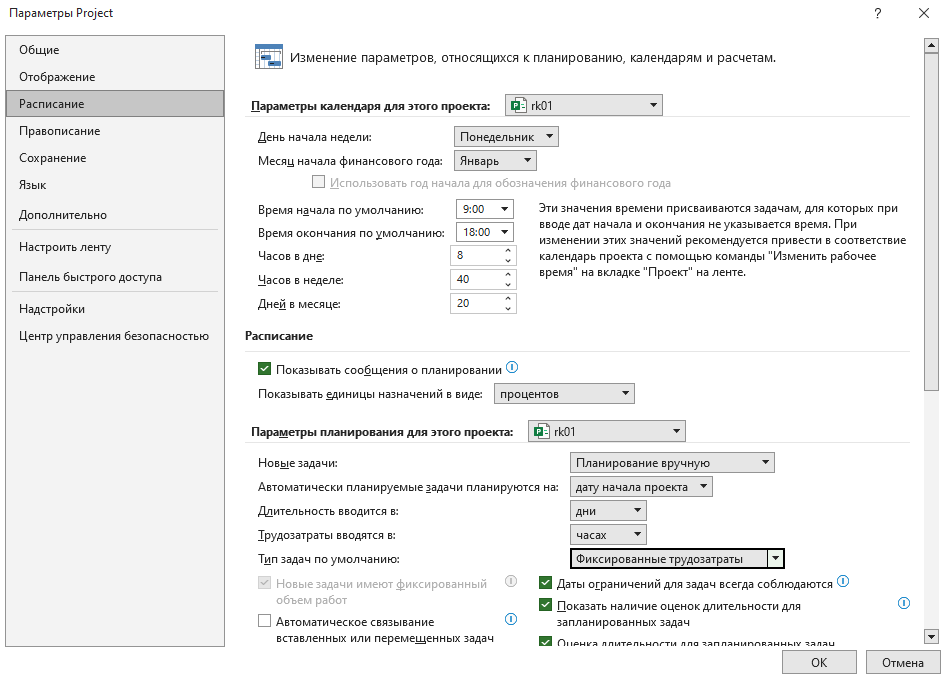
\includegraphics[scale=0.4, center]{rk1_task1_2}
\end{figure}

На вкладке Проект (Изменить рабочее время) добавим праздничные дни, попадающие на период реализации проекта.

\begin{figure}[h!]
	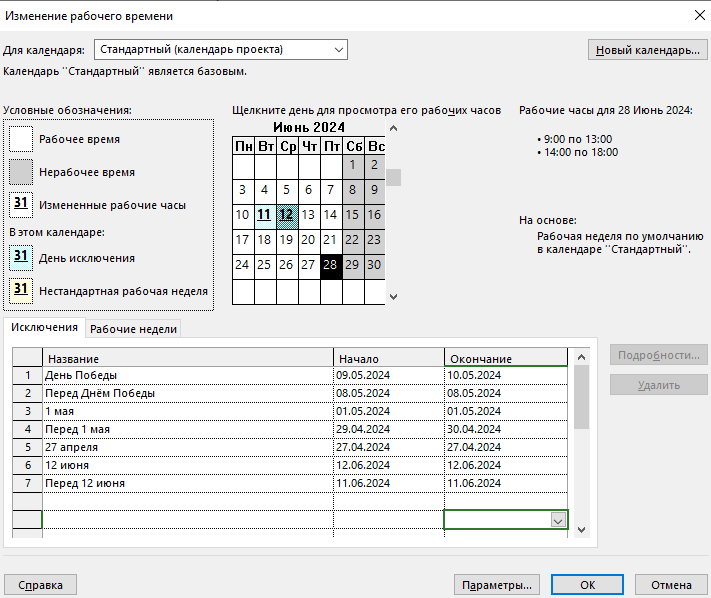
\includegraphics[scale=0.4, center]{rk1_task1_3}
\end{figure}

\subsection*{Задание 2}

Был осуществлён ввод задач в соответствии с заданием.

\begin{figure}[h!]
	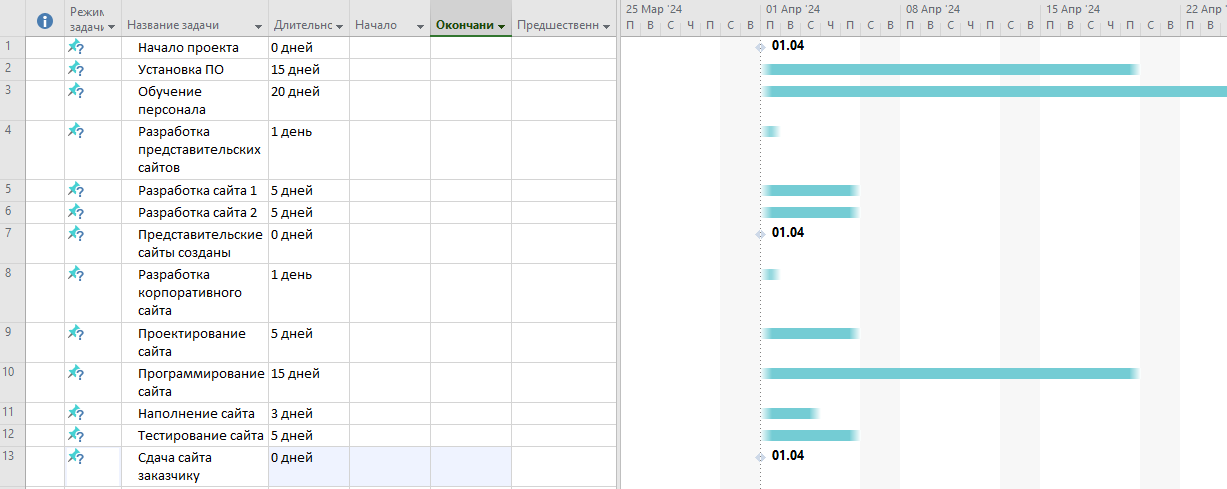
\includegraphics[scale=0.4, center]{rk1_task2_1}
\end{figure}
%\clearpage

\subsection*{Задание 3}

Была проведена группировка задач 5 -- 6 как подзадач задачи 4, а также задач 9 -- 12 как подзадачи задачи 8.

\begin{figure}[h!]
	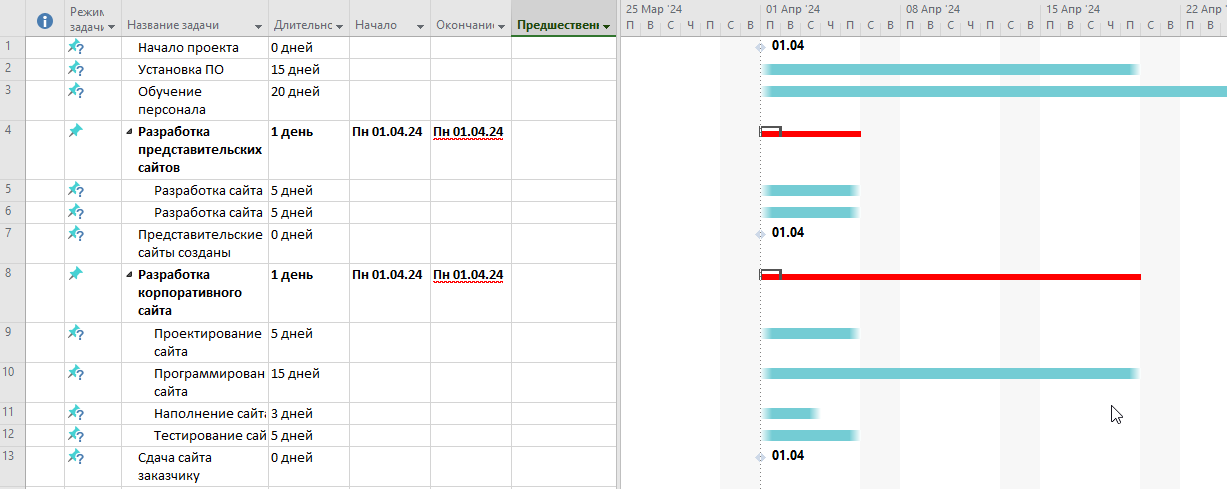
\includegraphics[scale=0.4, center]{rk1_task3_1}
\end{figure}
\clearpage

\subsection*{Задание 4}

Были установлено автоматическое планирование задач, а также добавлены связи между задачами посредством колонки Предшественники и получен итоговый результат:

\begin{figure}[h!]
	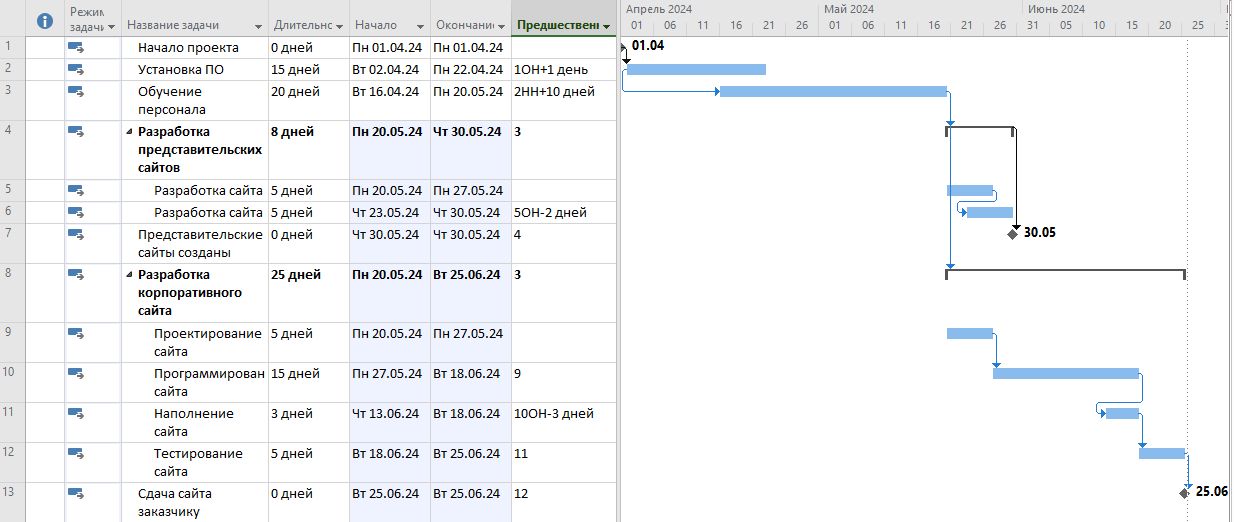
\includegraphics[scale=0.4, center]{rk1_task4_1}
\end{figure}

\subsection*{Задание 5}

Был создан список ресурсов согласно заданию:

\begin{figure}[h!]
	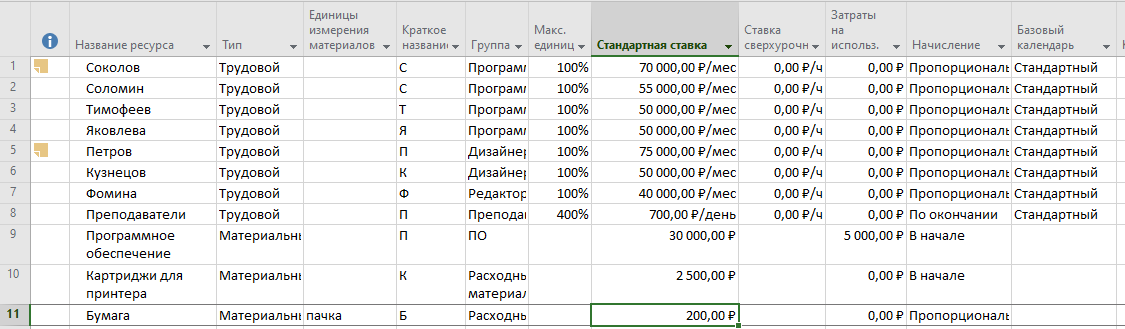
\includegraphics[scale=0.4, center]{rk1_task5_1}
\end{figure}

При помощи заметок были добавлены примечания о том, что Соколов явялется ведущим програмистом, а Петров --- руководителем дизайнерской группы. Расход бумаги в дальнейшем будет 3 пачки в месяц.

\begin{figure}[h!]
	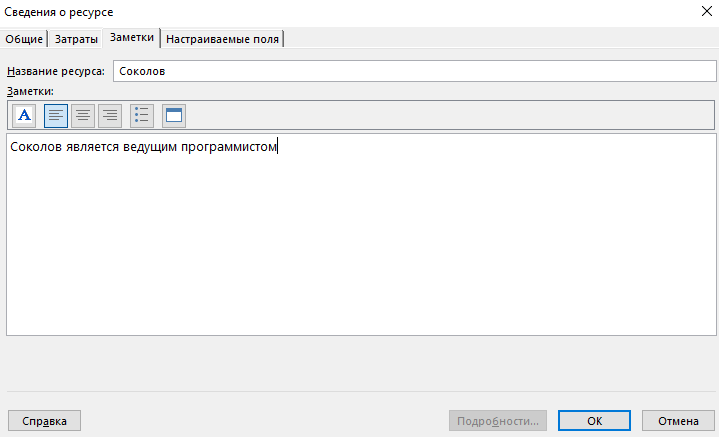
\includegraphics[scale=0.4, center]{rk1_task5_2}
\end{figure}

\begin{figure}[h!]
	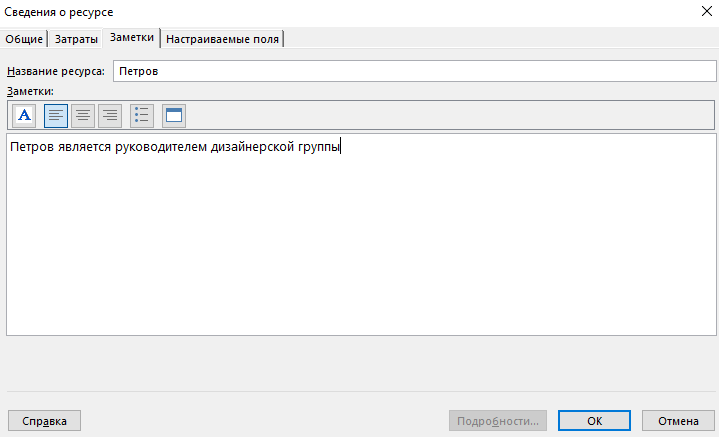
\includegraphics[scale=0.4, center]{rk1_task5_3}
\end{figure}

\subsection*{Задание 6}

Были назначены ресурсы задачам в соответствии с заданием, а также задачам 5 и 6 были установлены 500 рулей фиксированных затрат, а задаче 10 --- 10 000 рублей. Был сохранён исходный вариант проекта.

Дата завершения проекта 25 июня, стоимость проекта 674 650 рублей.

\begin{figure}[h!]
	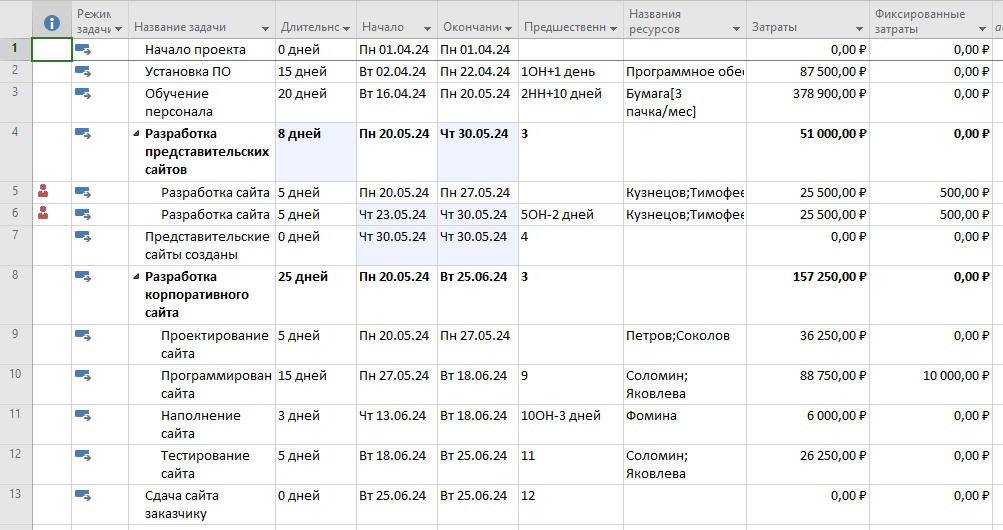
\includegraphics[scale=0.4, center]{rk1_task6_1}
\end{figure}

\clearpage

\subsection*{Задание 7}

Каждая из задач по разработке представительских сайтов была разбита на две подзадачи длительностью 2 и 3 дня соответственно (исполнители --- Кузнецов и Тимофеев соответственно).

\begin{figure}[h!]
	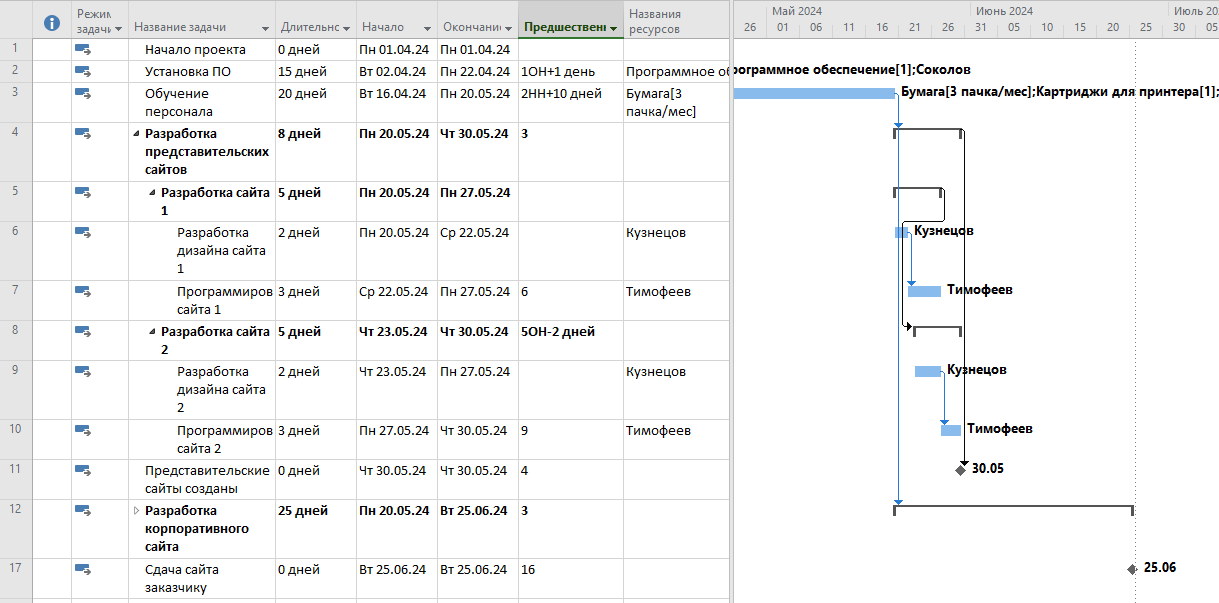
\includegraphics[scale=0.4, center]{rk1_task7_1}
\end{figure}

Это устранило перегрузку ресурсов, которая была ранее (поскольку задачи по разработке представительских сайтов пересекаются и имеют одинаковых исполнителей, у Кузнецова и Тимофеева была перегрузка).

Дата завершения проекта не изменилась (25 июня), а стоимость проекта изменилась с 674 650 рублей до 649 650 рублей (проект начал укладываться в бюджет, нагрузка на Кузнецова и Тимофеева уменьшилась).

\subsection*{Задание 8}

На момент начала задания 8 дата завершения 25 июня, а стоимость --- 649 650 рублей.

После назначения Соколова на задачу обучения персонала дата завершения 21 июня, а стоимость --- 679 068 рублей. В проекте присутствуют перегрузки (Соколов должен одновременно устанавливать ПО и обучаться как персонал).

После автоматического выравнивания и назначения Соколова на задачу обучения персонала только после того, как он завершит работы по установке ПО, дата завершения стала  1 июля, а стоимость осталась неизменной, 679 068 рублей. Перегрузок больше нет.

Для примменения разных профилей загрузки требуется зайти во вкладку Ресурсы, Использование ресурсов и выбрать у Соколова для конкретных задач нужный профиль загрузки. Был установлен профиль загрузки в начале для задачи установки ПО и загрузка в конце для задачи обучения персонала. 

\begin{figure}[h!]
	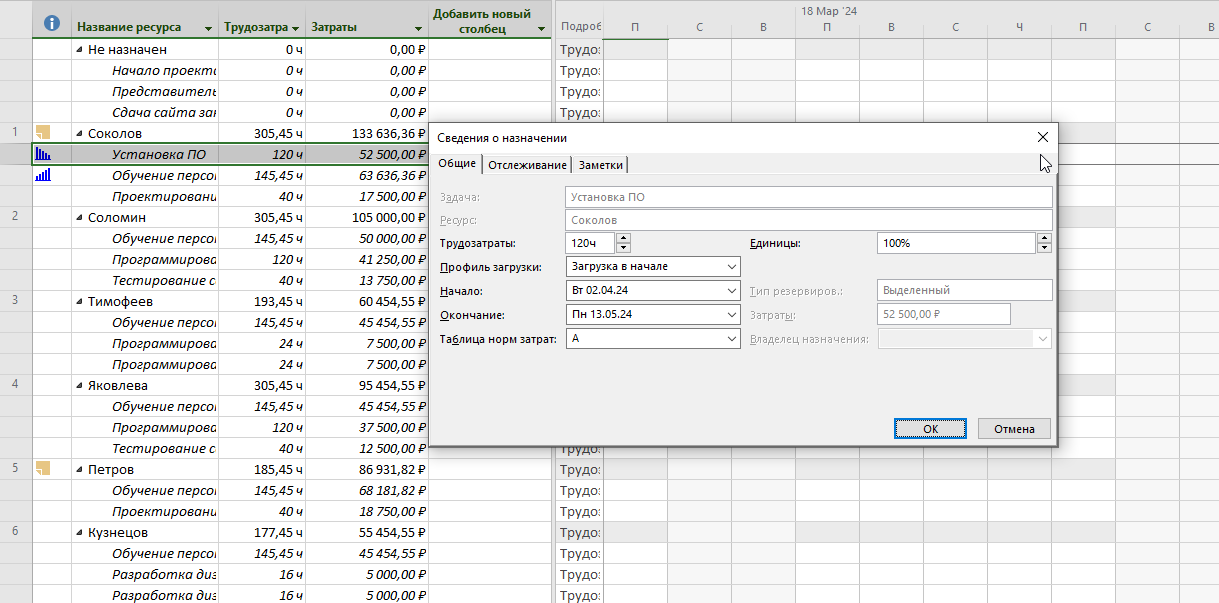
\includegraphics[scale=0.4, center]{rk1_task8_4}
\end{figure}


После этого дата завершения проекта стала 9 июля, стоимость не изменилась.

Из двух вариантов назначения Соколова на задачу обучения персонала наиболее предпочтителен вариант с плоским профилем нагрузки (с ним дата окончания 1 июля).

Решение назначить Соколова на задачу обучения персонала привело увеличению длительности проекта (дата окончания сдвинулась с 21 июня на 1 июля), а стоимость проекта увеличилась (с 649 650 до 679 068 рублей). Выберем наиболее оптимальный способ использования ресурсов в проекте.

\subsection*{Задание 9}

Выведем критический путь проекта:

\begin{figure}[h!]
	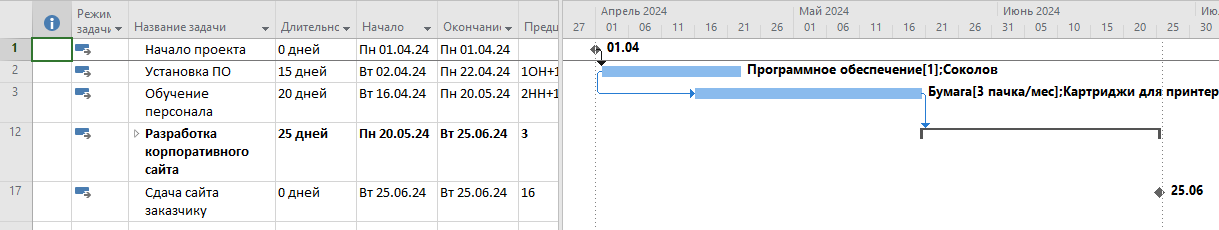
\includegraphics[scale=0.4, center]{rk1_task9_1}
\end{figure}

Есть возможность оптимизировать критический путь по времени (например, назначить дополнительные ресурсы на задачи разработки корпоративного сайта), однако это будет нецелесообразно, поскольку тогда бюджет проекта будет превышен (сейчас он составляет 649 650 рублей).

Был сохранён базовый план проекта.
\begin{figure}[h!]
	
\includegraphics[scale=0.6, center]{rk1_task9_2}
\end{figure}

\subsection*{Задание 10}

Установим дату отчёта 1 июня:

\begin{figure}[h!]
	
\includegraphics[scale=0.6, center]{rk1_task10_1}
\end{figure}

Актуализируем информацию о задачах следующим образом: обучение персонала заняло на 1 день меньше, чем ожидалось, а задача ''Разработка дизайна 1'' заняла не 2, а 3 дня. 

С 30 мая программиста Тимофеева мобилизируют, он доступен до 30 мая:

\begin{figure}[h!]
	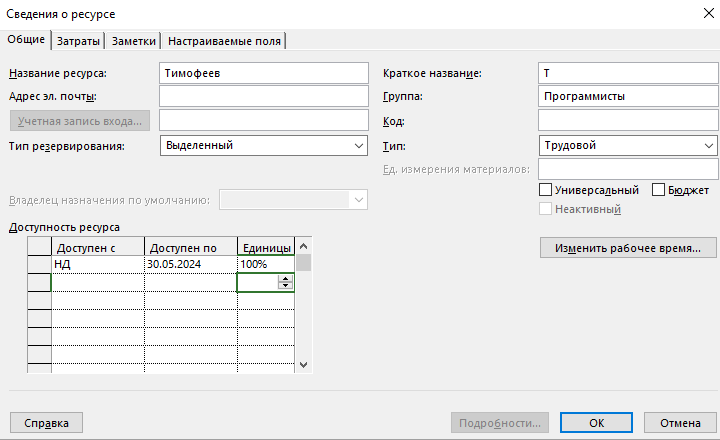
\includegraphics[scale=0.6, center]{rk1_task10_2}
\end{figure}

Чтобы его задача была выполнена в срок, поставим Яковлеву на задачу ''Программирование сайта 2''. Итоговые даты в виде таблицы и в виде диаграммы Ганта с отклонениями от базового плана:

\begin{figure}[h!]
	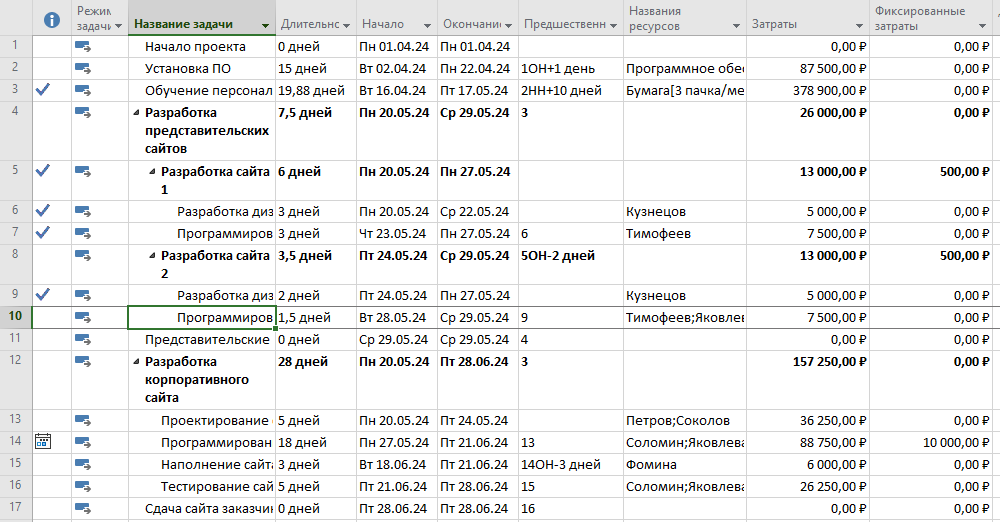
\includegraphics[scale=0.4, center]{rk1_task10_3}
\end{figure}

\begin{figure}[h!]
	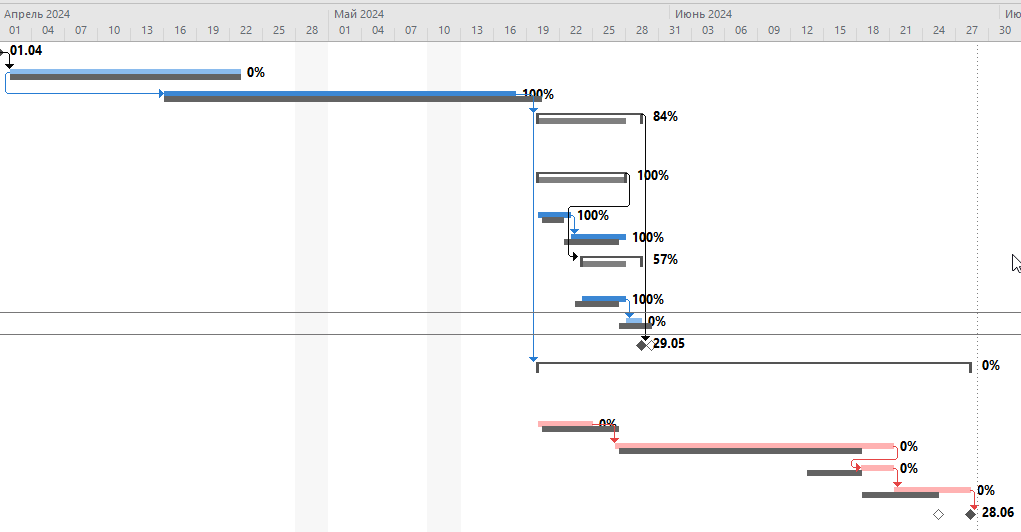
\includegraphics[scale=0.4, center]{rk1_task10_4}
\end{figure}
\clearpage
Выведем на экран линию прогресса:

\begin{figure}[h!]
	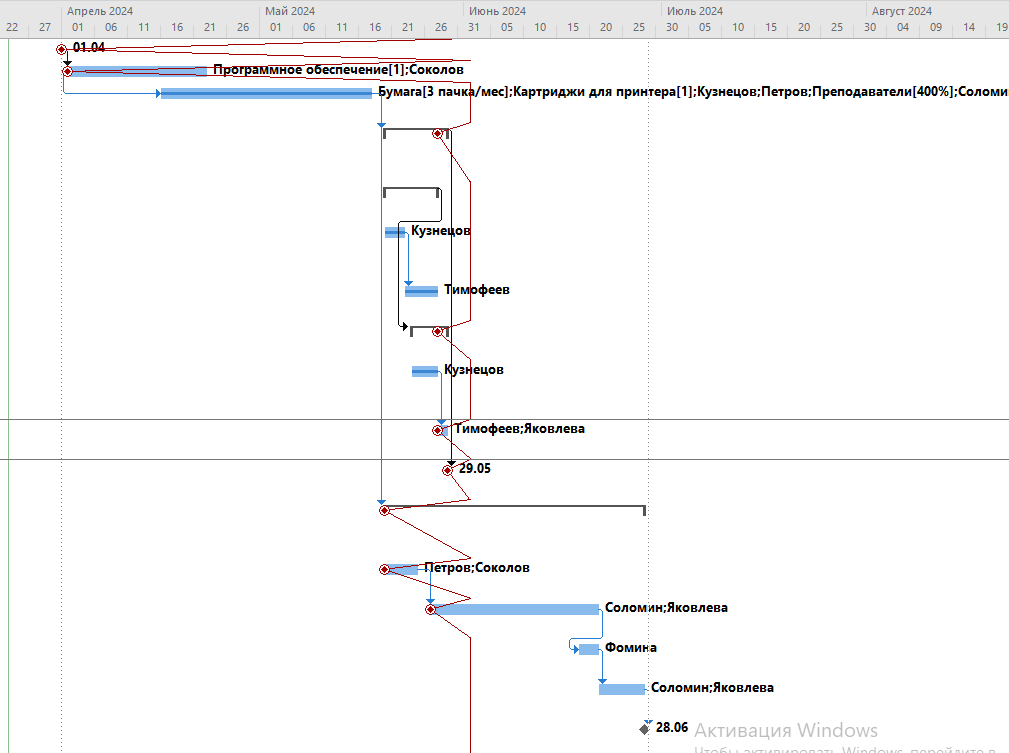
\includegraphics[scale=0.4, center]{rk1_task10_5}
\end{figure}

\clearpage

Выведем таблицу освоенного объёма: 

\begin{figure}[h!]
	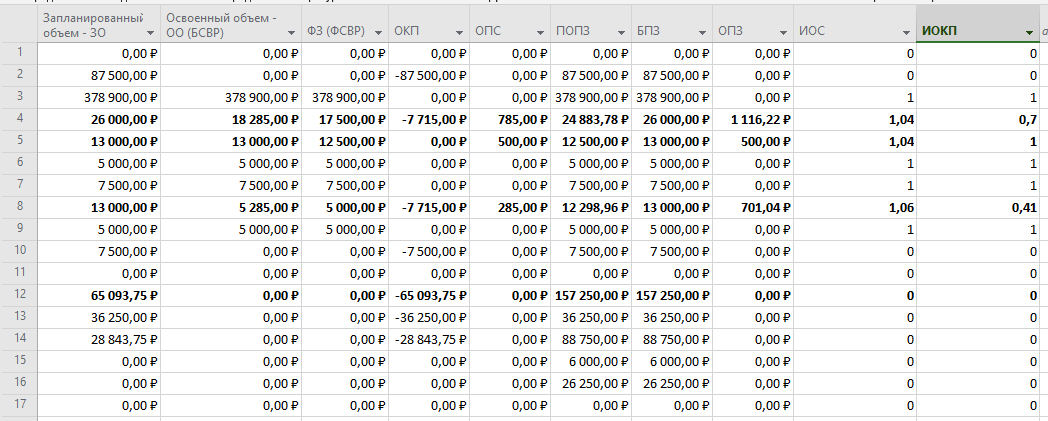
\includegraphics[scale=0.4, center]{rk1_task10_6}
\end{figure}

ОКП отрицательно, что показывает, что проект выполняется с задержкой (а именно дата завершения сместилас с 25 июня на 28), а ОПС и ОПЗ положительны, что означает, что проект укладывается в бюджет. Коэффициенты ИОС (больше 1) и ИОКП (меньше 1) указывают на то же.

\clearpage

\section*{Заключение}

В ходе выполнения рубежного контроля при помощи программы MS Project 2016 был создан проект и выполнено планирование работы Internet-компании. Была произведена настройка рабочей среды проекта, создан и структурирован список задач, установлены связи между задачами, создан список ресурсов, которые были назначены задачам, проведена оптимизация загрузки ресурсов с разбиением задач на подзадачи, был уточнён план проекта на 1 июня, осуществлён контроль за реализацией проекта.

В результате выяснилось, что проект укладывается в изначальные сроки: дата завершения 28 июня, а также в бюджет (649 650 рублей).
